% !TeX root = ../dokumentation.tex

\chapter{Technische Umsetzung}


\section{Architektur}
Um unsere Plattform potenziellen Nutzern zugänglich zu machen und bestimmte Teile unseres Workflows\footnote{Arbeitsablauf} zu Automatisieren, hosten wir unsere Architektur in einer Cloud Umgebung.
Dabei läuft unsere Architektur auf der Kontainer Orchestrierungs Plattform Kubernetes, für welches wir die leichgewichtige (und leichter zu verwaltende) Variante \textit{k3s}~\parencite{web/k3s} verwenden.
Auf diesem Kubernetes System werden \ac{CI/CD} Plattformen gehosted und unsere Applikation sowie deren Abhängigkeiten. Dadruch sind wir nicht an öffentlich-kostenfreie System limitiert und können unsere
System perfekt auf unseren Workflow und die Applikation anpassen.

\subsection{Übersicht der Services}
Unser Produkt ist in mehrere Services aufgeteilt. Die Services sind \textit{Core-Service}, \textit{Polling-Service} und das \textit{Frontend}.
Desweiteren gibt es eine \textit{PostgreSQL Datenbank} und eine \textit{Keycloak} Instanz. Die letzten beiden Services sind Abhänigkeiten von unseren entwickelten Services.
Die Datenbank wird dafür verwendet um Daten wie RSS-Feeds und Artikel zu speichern.
Keycloak wird dafür verwendet um den \textit{Core-Service} und das \textit{Frontend} abzusichern und die Benutzer zu verwalten.
Die Hauptaufgabe des \textit{Core-Services} ist es RSS-Feeds und Artikel zur Verfügung zu stellen, dies geschieht mittels \textit{GraphQL}. Desweiteren bietet er die Möglichkeit
RSS-Feeds anzulegen und Abonnents, Favouriten und Lesezeichen eines Benutzers zu verwalten.
Der \textit{Polling-Service} ist für die automatische Datenabfrage von RSS-Feeds und deren Artikel zuständig. Diese werden anschließend in der Datenbank gespeichert.
Das \textit{Frontend} ist die Endschnittstelle unseres Produkts zu dem Benutzer.
Es wird dafür verwendet um die Daten des \textit{Core-Services} dem Benutzer zugänglich zu machen.
Das folgenden Diagramm veranschautlicht die Skiosa Service-Architektur. Die Sevices mit den gestrichelten Linien sind die Abhängigkeiten.
\begin{figure}[!htbp]
    \centering    
    \usetikzlibrary{positioning}
    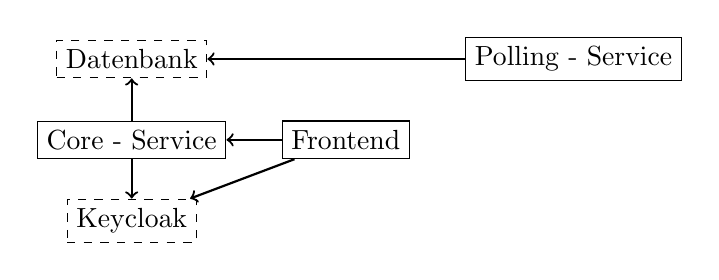
\begin{tikzpicture}
        \matrix [column sep=7mm, row sep=5mm] {
            \node (database) [draw, shape=rectangle, dashed] {Datenbank}; &&
            \node (polling_service) [draw, shape=rectangle] {Polling - Service}; \\
            \node (core_service) [draw, shape=rectangle] {Core - Service}; &
            \node (frontend) [draw, shape=rectangle] {Frontend}; \\
            \node (keycloak) [draw, shape=rectangle, dashed] {Keycloak}; \\
            };
            \draw[->, thick] (core_service) -- (database);
            \draw[->, thick] (frontend) -- (core_service);
            \draw[->, thick] (polling_service) -- (database);
            \draw[->, thick] (core_service) -- (keycloak);
            \draw[->, thick] (frontend) -- (keycloak);
        \end{tikzpicture}        
\caption{Diagramm – Darstellung der Service Architektur}
\end{figure}

\subsection{CI/CD Infrastrukture}
Um Code Qualität zu gewährleisten, wurde eine \ac{CI/CD} Infrastruktur entwickelt.
Diese ermöglicht es uns automatisiert Tests wie Unit und Integration Tests auszuführen und nach jeder Änderung aktuelle Versionen der Software zu veröffentlichen.
Da zum Beispiel eine neue veröffentlichung bei Änderungen auf der Master Branch stattfinden sollen, gibt es drei verschieden \ac{CI/CD} Pipelines.
Eine die nur Unit-Tests ausführt, eine die komplexe Tests ausführt und eine die eine neue Version veröffentlicht.

\subsubsection{Übersicht der Standard \ac{CI}-Pipline}
Die Standard \ac{CI}-Pipeline wird bei jedem Commit der nicht auf dem Master Branch stattfindet ausgeführt. Dabei hat die Standard Pipeline den geringsten Umfang and Aufgaben.
Diese führt nur die Unit-Tests aus, dazu muss der Code gecloned und alle Dependencies installiert werden. Somit sind direkt Fehler schon früh erkennbar, wenn diese Pipeline fehlschlägt.
\begin{figure}[!htbp]
    \centering    
    \usetikzlibrary{positioning}
    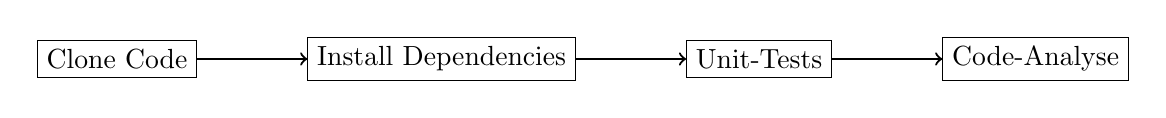
\begin{tikzpicture}
        \matrix [column sep=7mm, row sep=5mm] {
            \node (clone) [draw, shape=rectangle] {Clone Code}; &&
            \node (npm_setup) [draw, shape=rectangle] {Install Dependencies}; &&
            \node (unit_test) [draw, shape=rectangle] {Unit-Tests}; &&
            \node (sonar) [draw, shape=rectangle] {Code-Analyse}; \\
            };
            \draw[->, thick] (clone) -- (npm_setup);
            \draw[->, thick] (npm_setup) -- (unit_test);
            \draw[->, thick] (unit_test) -- (sonar);
        \end{tikzpicture}        
\caption{Diagramm – Darstellung der Standard \ac{CI}-Pipeline}
\end{figure}

\subsubsection{Übersicht der Pull-Request \ac{CI}-Pipline}
Die Pull-Request \ac{CI}-Pipeline wird ausgeführt sobald ein Pull-Request erstellt wird. Ihr Ziel ist es den jeweiligen Reviewer zu unterstützen, indem sie Tests und Code-Analyse durchführt.
Die Ergebnisse der Code Analyse werden direkt auf der Pull-Request Seite dargestellt. Sollten diese nicht den mindestanforderungen entsprechen, wird der Pull-Request dadurch blockiert.
Die Pipeline beinhaltet die selben Schritte wie die Standard Pipeline, sie erweitert diese lediglich um Integration-Tests.
\begin{figure}[!htbp]
    \centering    
    \usetikzlibrary{positioning}
    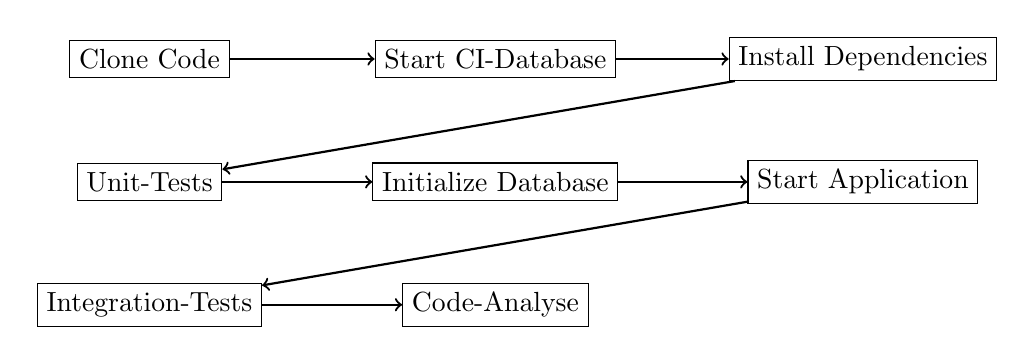
\begin{tikzpicture}
        \matrix [column sep=7mm, row sep=10mm] {
            \node (clone) [draw, shape=rectangle] {Clone Code}; &&
            \node (database) [draw, shape=rectangle] {Start \ac{CI}-Database}; &&
            \node (npm_setup) [draw, shape=rectangle] {Install Dependencies}; \\
            \node (unit_test) [draw, shape=rectangle] {Unit-Tests}; &&
            \node (init_db) [draw, shape=rectangle] {Initialize Database}; &&
            \node (start_app) [draw, shape=rectangle] {Start Application}; \\
            \node (int_test) [draw, shape=rectangle] {Integration-Tests}; &&
            \node (sonar) [draw, shape=rectangle] {Code-Analyse}; \\
            };
            \draw[->, thick] (clone) -- (database);
            \draw[->, thick] (database) -- (npm_setup);
            \draw[->, thick] (npm_setup) -- (unit_test);
            \draw[->, thick] (unit_test) -- (init_db);
            \draw[->, thick] (init_db) -- (start_app);
            \draw[->, thick] (start_app) -- (int_test);
            \draw[->, thick] (int_test) -- (sonar);
        \end{tikzpicture}
\caption{Diagramm – Darstellung der Pull-Request \ac{CI}-Pipeline}
\end{figure}

\subsubsection{Übersicht der Master \ac{CI}-Pipline}
Die Master \ac{CI}-Pipeline wird bei einen Commit auf den Master Branch ausgeführt. Dabei hat die Pipeline die Aufgabe den neuen Code auszurollen und sommit live zu bringen.
Zur Sicherheit werden auch wieder die Unit-Tests ausgeführt, damit auch wirklich sichergestellt wird, dass der Code lauffähig ist. Anschließend wird ein neues Docker-Image gebaut
welches dann in der Docker-Registry gespeichert wird. Nach erfolgreichem bauen des Images, wird die neue Image-Version in das Kubernetes-Depyoment geschrieben. Denn ArgoCD~\parencite{web/argocd} unser \ac{CD} Tool
erkennt automatisch Änderungen an den Kubernetes-Deployments und übernimmt diese. Somit sind die Code Änderungen an der Software in wenigen Minuten live ausgerollt.
\begin{figure}[!htbp]
    \centering    
    \usetikzlibrary{positioning}
    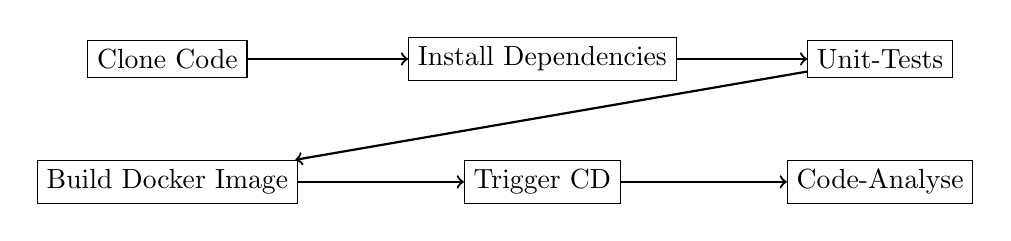
\begin{tikzpicture}
        \matrix [column sep=7mm, row sep=10mm] {
            \node (clone) [draw, shape=rectangle] {Clone Code}; &&
            \node (npm_setup) [draw, shape=rectangle] {Install Dependencies}; &&
            \node (unit_test) [draw, shape=rectangle] {Unit-Tests}; \\
            \node (docker_build) [draw, shape=rectangle] {Build Docker Image}; &&
            \node (trigger_cd) [draw, shape=rectangle] {Trigger \ac{CD}}; &&
            \node (sonar) [draw, shape=rectangle] {Code-Analyse}; \\
            };
            \draw[->, thick] (clone) -- (npm_setup);
            \draw[->, thick] (npm_setup) -- (unit_test);
            \draw[->, thick] (unit_test) -- (docker_build);
            \draw[->, thick] (docker_build) -- (trigger_cd);
            \draw[->, thick] (trigger_cd) -- (sonar);
        \end{tikzpicture}
\caption{Diagramm – Darstellung der Master \ac{CI}-Pipeline}
\end{figure}

\section{Mockups}

\subsection{Aktivitätsdiagramme}
Das Aktivitätsdiagram der Loginseite ist in Abbildung~\ref{fig:umlActivityLogin.png} dargestellt.
Auf der Seite kann man sich entweder direkt mit Username und Passwort anmelden oder auf registrieren klicken.
Sind die Anmeldedaten korrekt wird man eingeloggt, sind die Anmeldedaten fehlerhaft können diese korrigiert werden.
\begin{figure}
    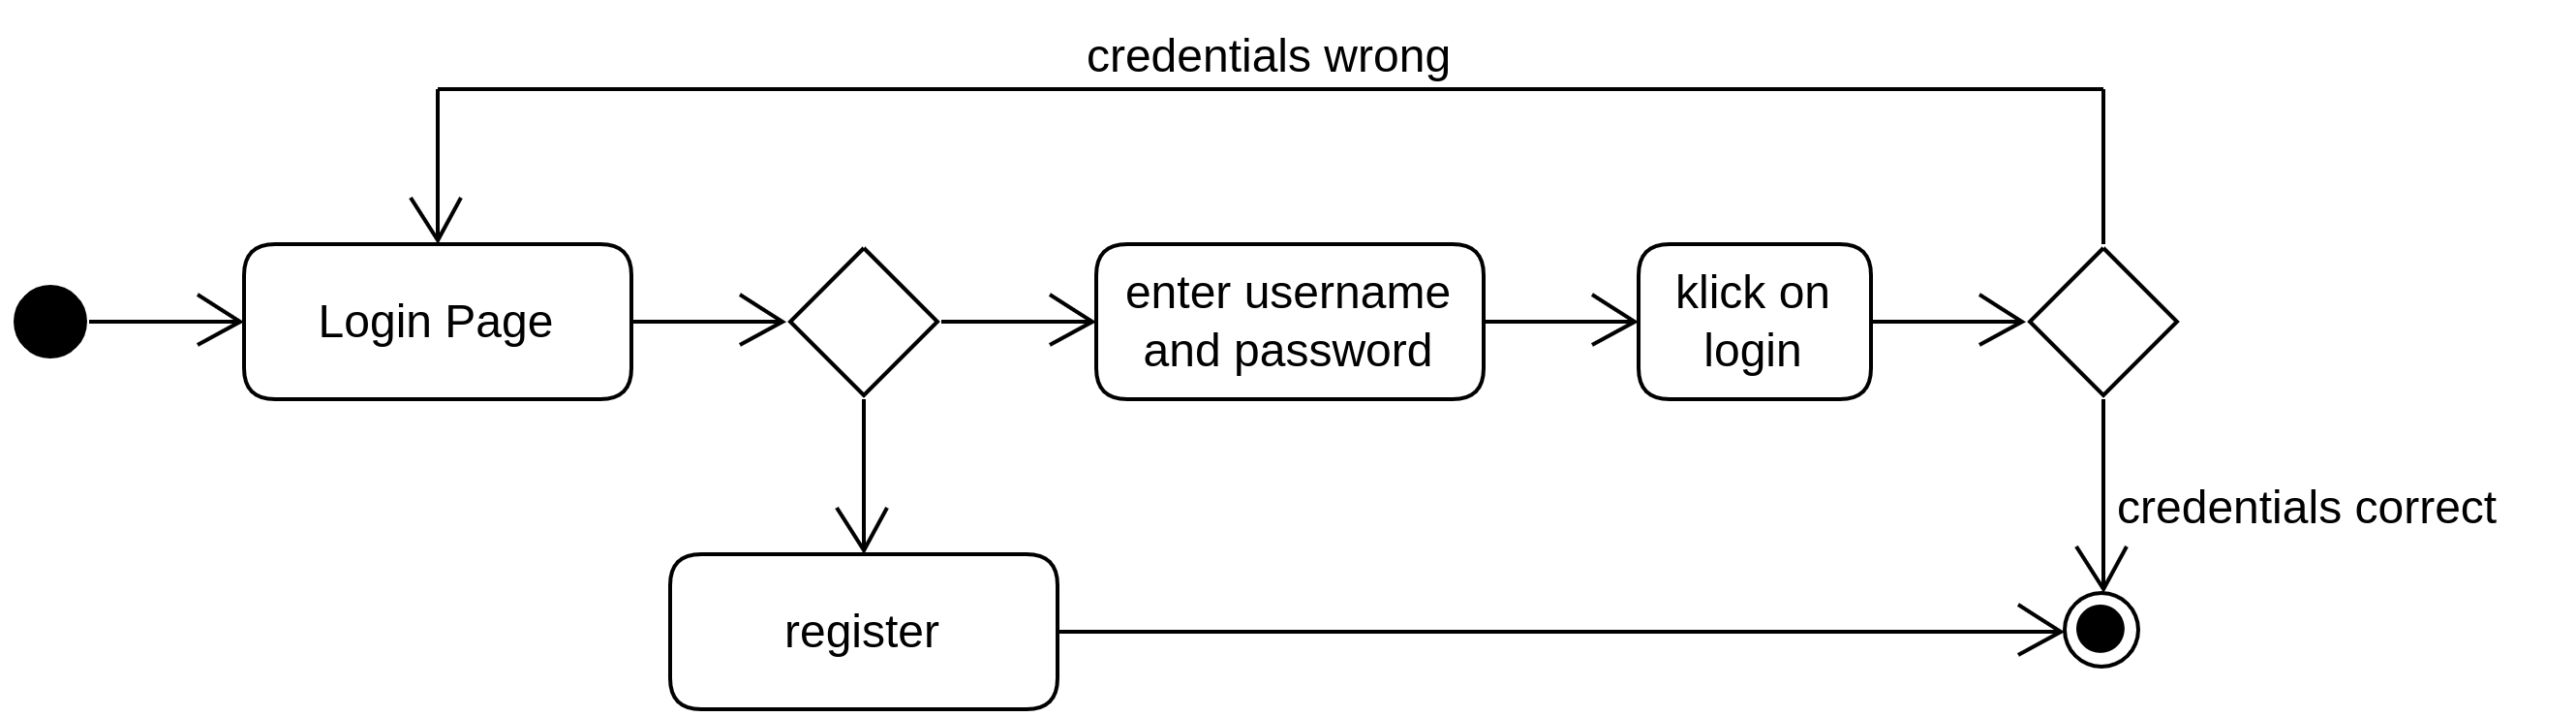
\includegraphics[width=\linewidth]{umlActivityLogin.png}
    \caption{Aktivitätsdiagramm der Loginseite}
    \label{fig:umlActivityLogin.png}
\end{figure}

In Abbildung~\ref{fig:umlActivityRegister.png} wird die Registrierungsseite beschrieben.
Auf der Seite müssen Daten, wie Vorname, Nachname, E-Mail, Benutzername, sowie Passwort und dessen Wiederholung eingetragen werden.
Sind die Registrierungsdaten korrekt, bzw. nicht bereits registriert (z.B. Benutzername) kann mit Bestätigung auf registrieren ein User angelegt werden.
Zu jedem Zeitpunkt kann die Registrierung abgebrochen und zur Loginseite zurückgekehrt werden.
\begin{figure}
    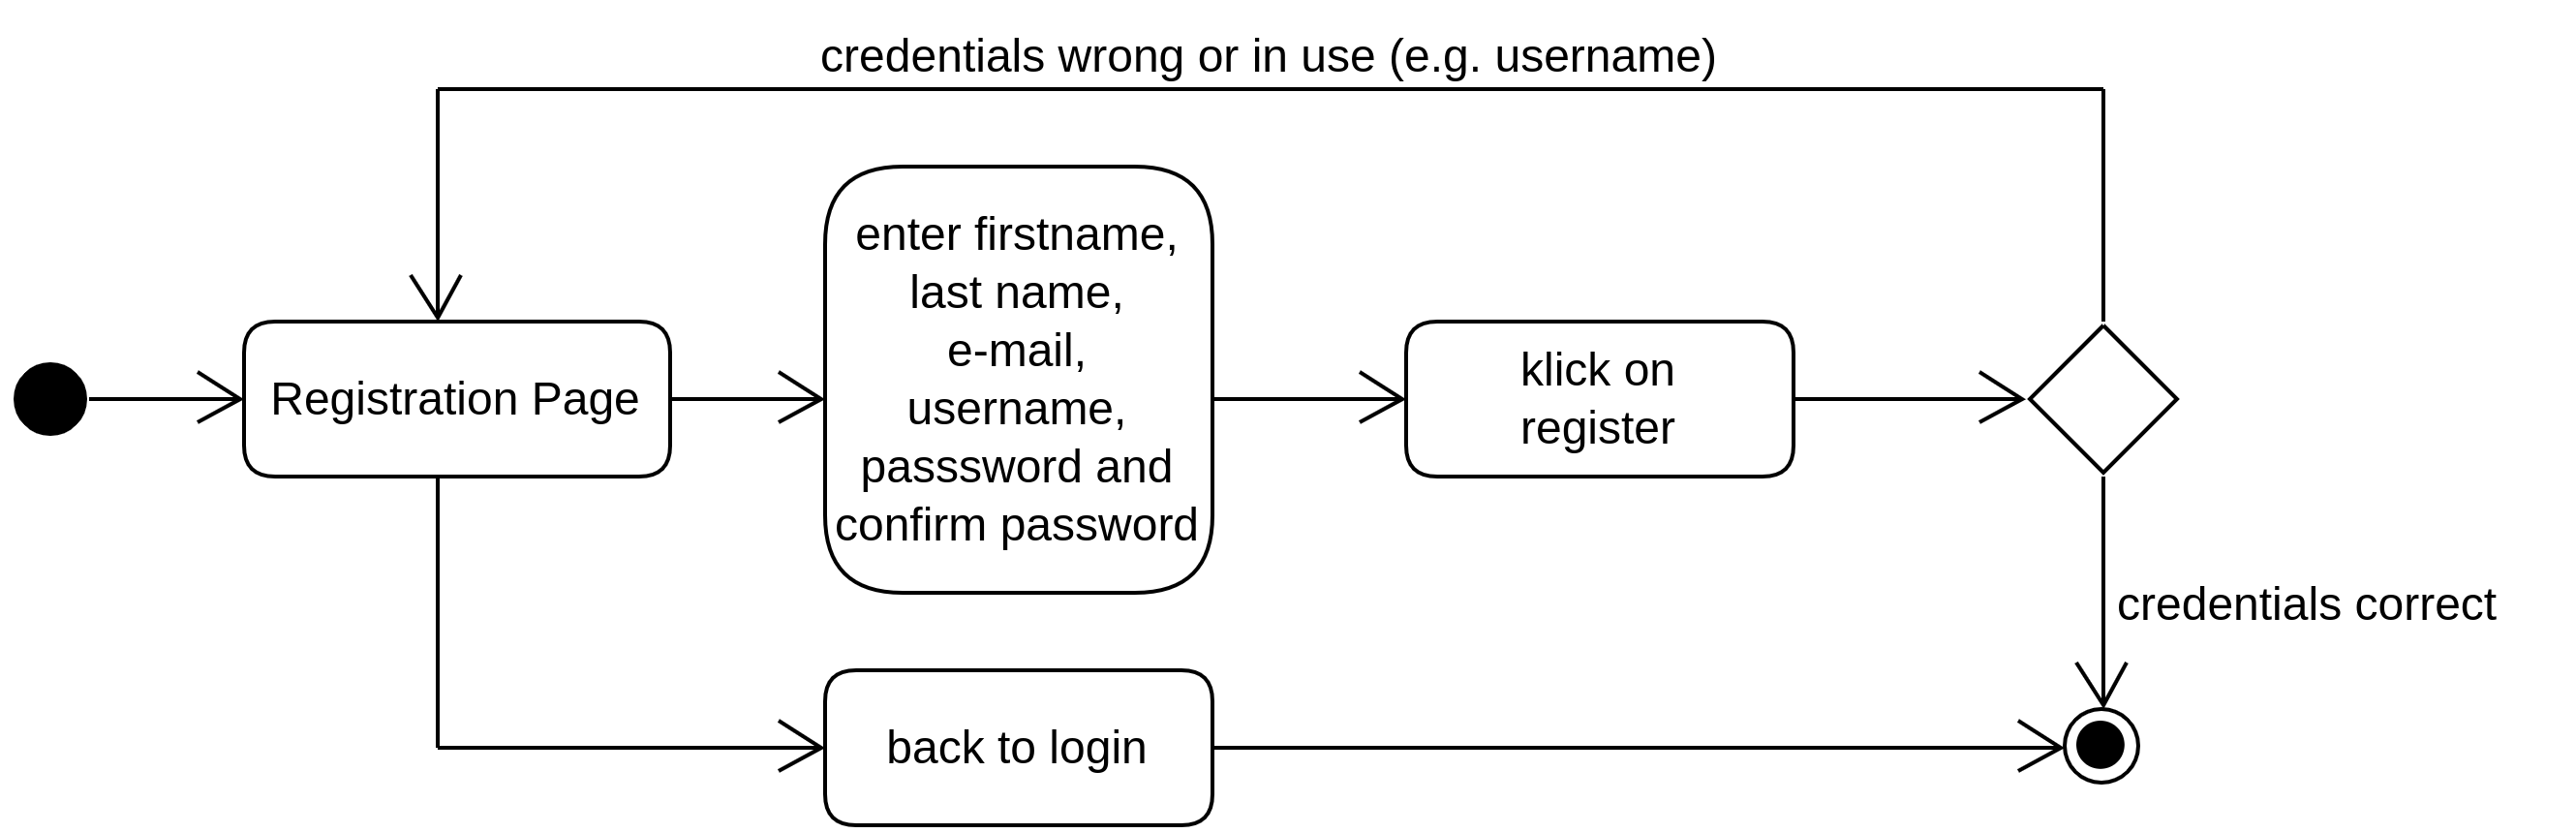
\includegraphics[width=\linewidth]{umlActivityRegister.png}
    \caption{Aktivitätsdiagramm der Registrierungsseite}
    \label{fig:umlActivityRegister.png}
\end{figure}

Die Seitenleiste ist auf jeder Seite mit Außnahme Login- und Registrierungsseite, sowie während des Pop-ups zum Hinzufügen eines Feeds erreichbar.
In Abbildung~\ref{fig:umlActivitySidebar.png} werden die möglichen Aktionen der Seitenleiste dargestellt.
Von dieser kann direkt zwischen Dark- und Light-Mode umgeschalten werden. Zudem kann man sich einloggen
oder falls bereits geschehen auf die Einstellungen gewechselt werden. Die Schaltfläche des Login wird nach erfolgreichem Login auf Settings geändert.
Unter der Voraussetzung, dass der Benutzer eingeloggt ist, kann direkt zu den
Empfehlungen, den Lesezeichen und den Abonnements gewechselt werden. Zusätzlich kann direkt ein neuer RSS Feed hinzugefügt werden.
\begin{figure}
    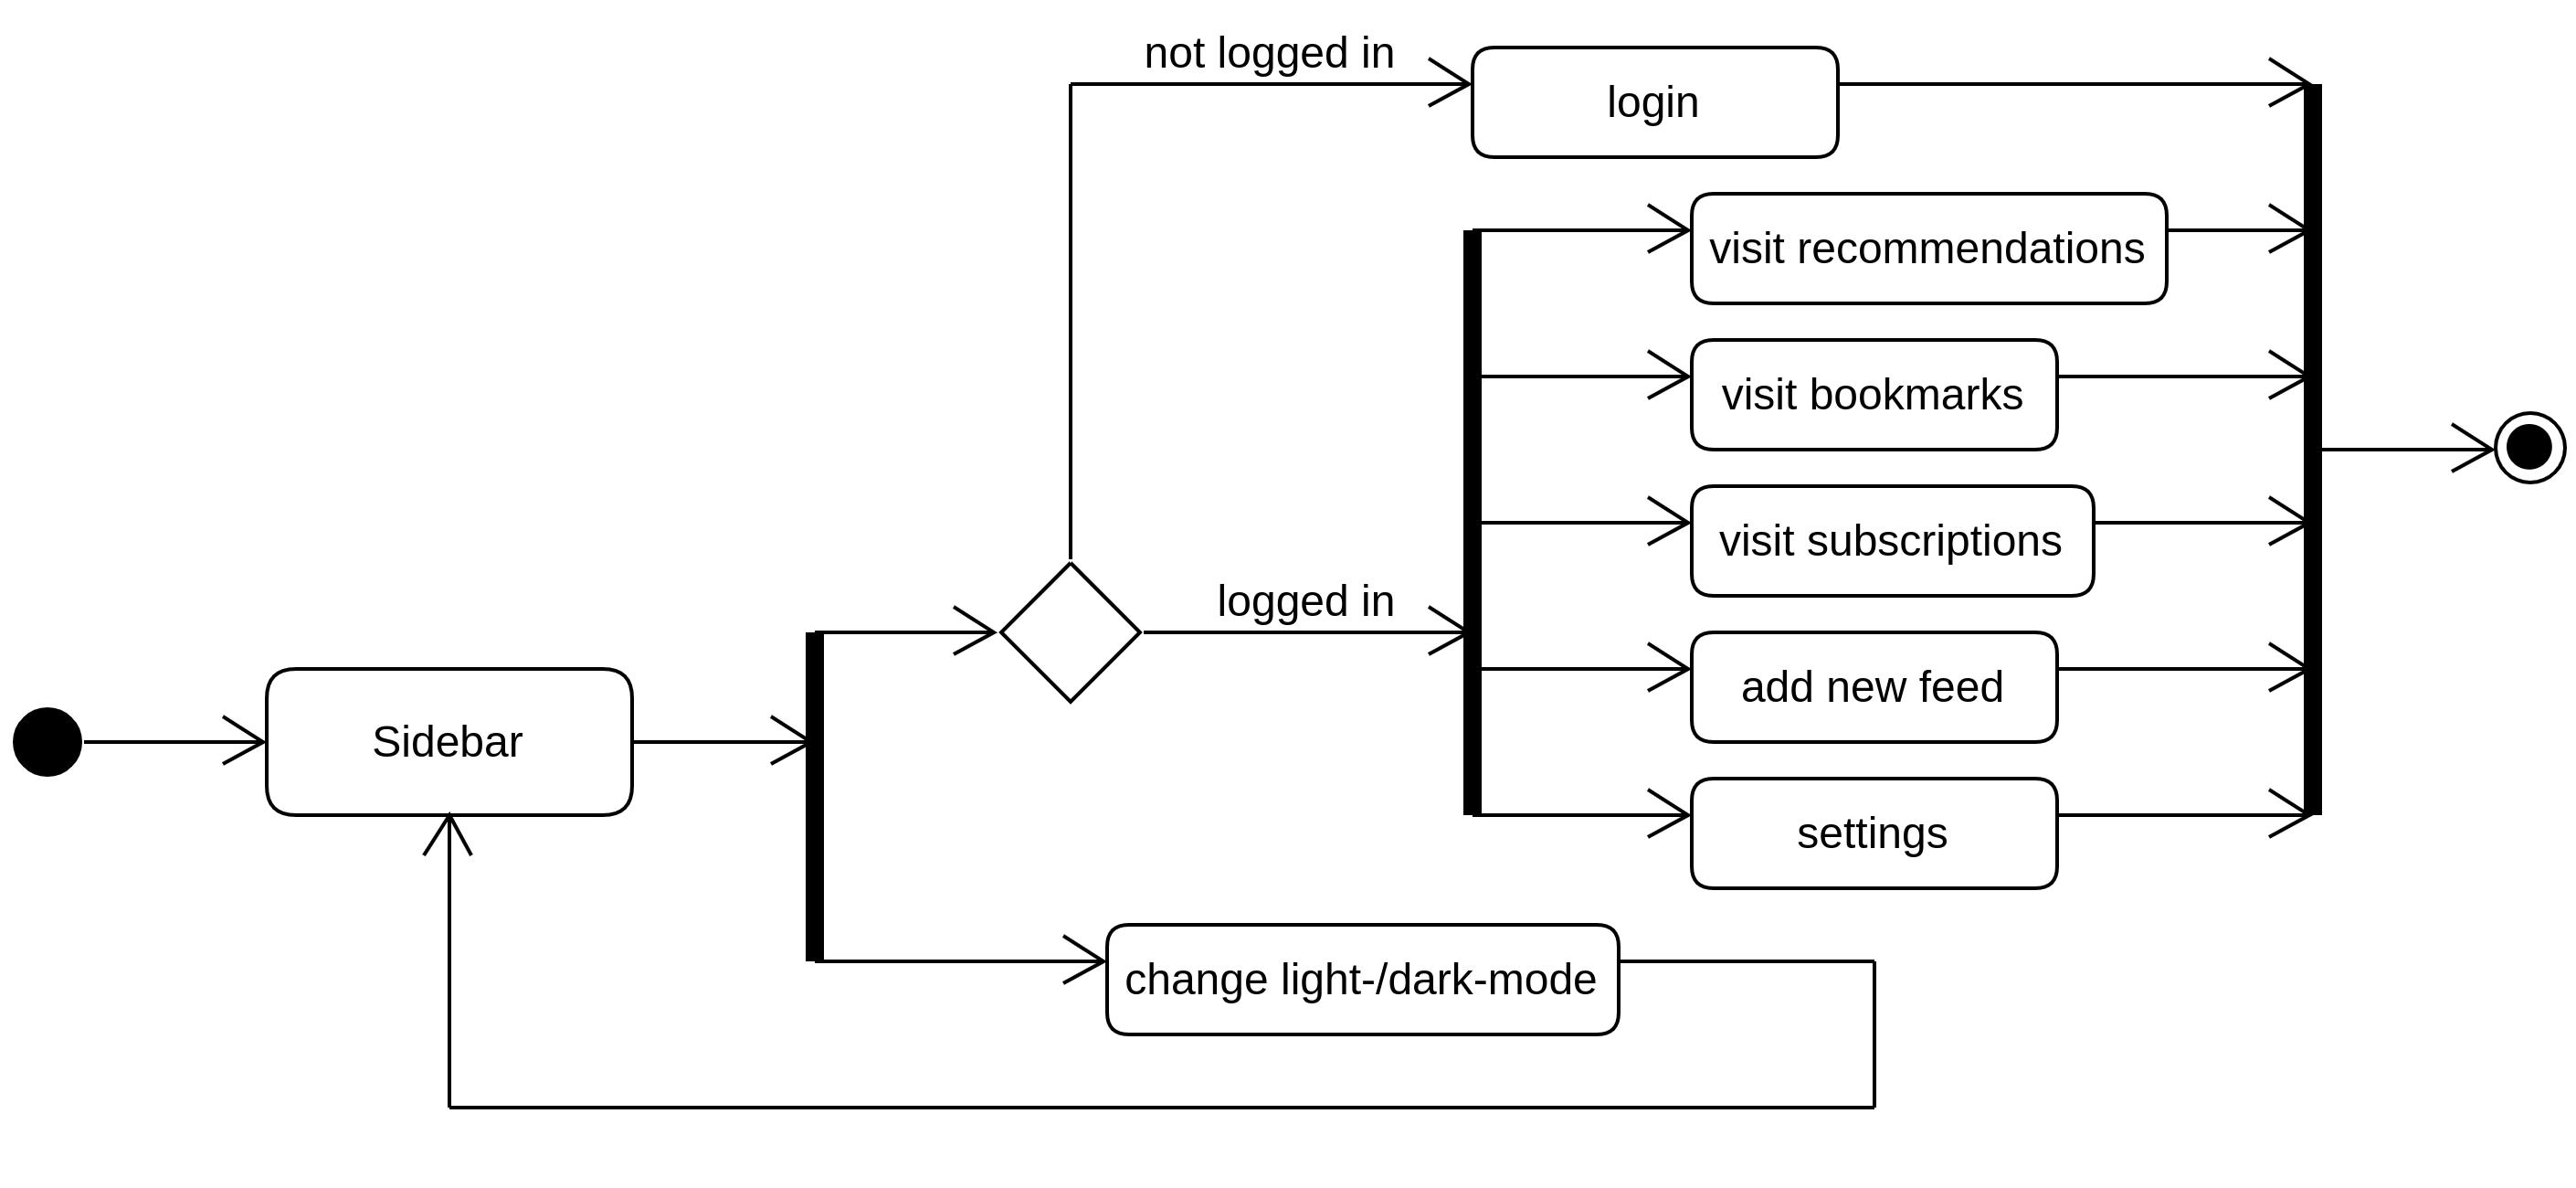
\includegraphics[width=\linewidth]{umlActivitySidebar.png}
    \caption{Aktivitätsdiagramm der Seitenleiste}
    \label{fig:umlActivitySidebar.png}
\end{figure}

Auf der Übersichtsseite können empfohlene Feeds oder empfohlene Artikel besucht werden.
Das Aktivitätsdiagramm ist in Abbildung~\ref{fig:umlActivityOverview.png} dargestellt.
\begin{figure}
    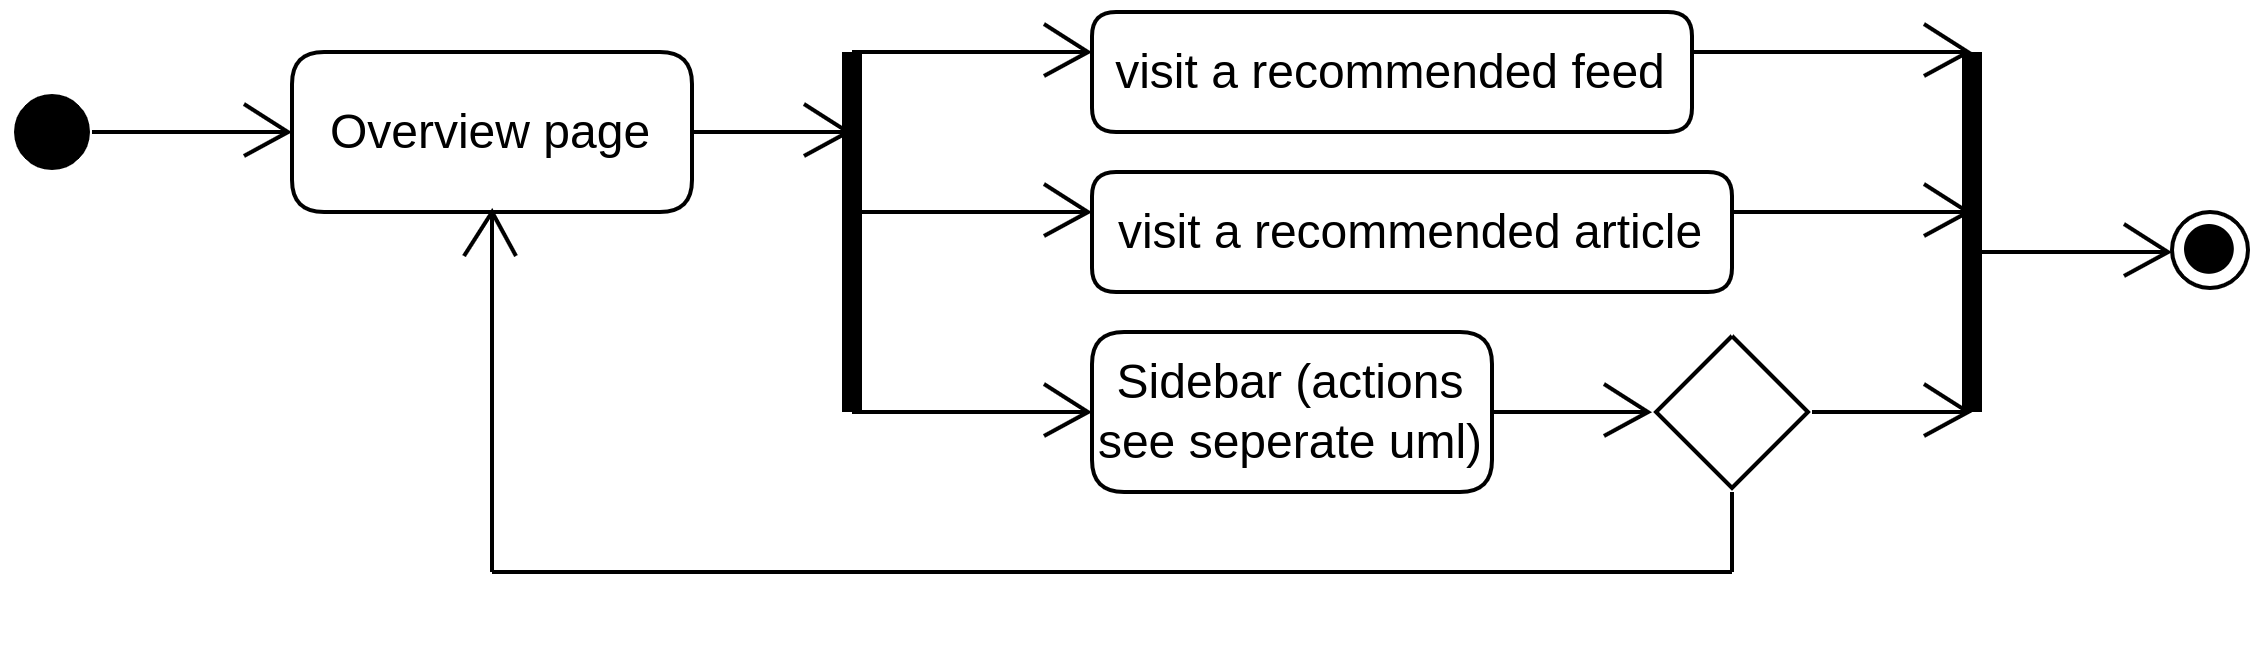
\includegraphics[width=\linewidth]{umlActivityOverview.png}
    \caption{Aktivitätsdiagramm der Übersichtsseite}
    \label{fig:umlActivityOverview.png}
\end{figure}

In Abbildung~\ref{fig:umlActivityFeed.png} werden die möglichen Aktionen auf der Feedseite dargestellt.
Der aufgerufene Feed kann abonniert und deabonniert werden. Im Feed kann gefiltert und/oder gesucht werden.
Einzelne Artikel können als Lesezeichen gespeichert oder geliked werden. Per Klick auf den Artikel kann dieser aufgerufen werden.
\begin{figure}
    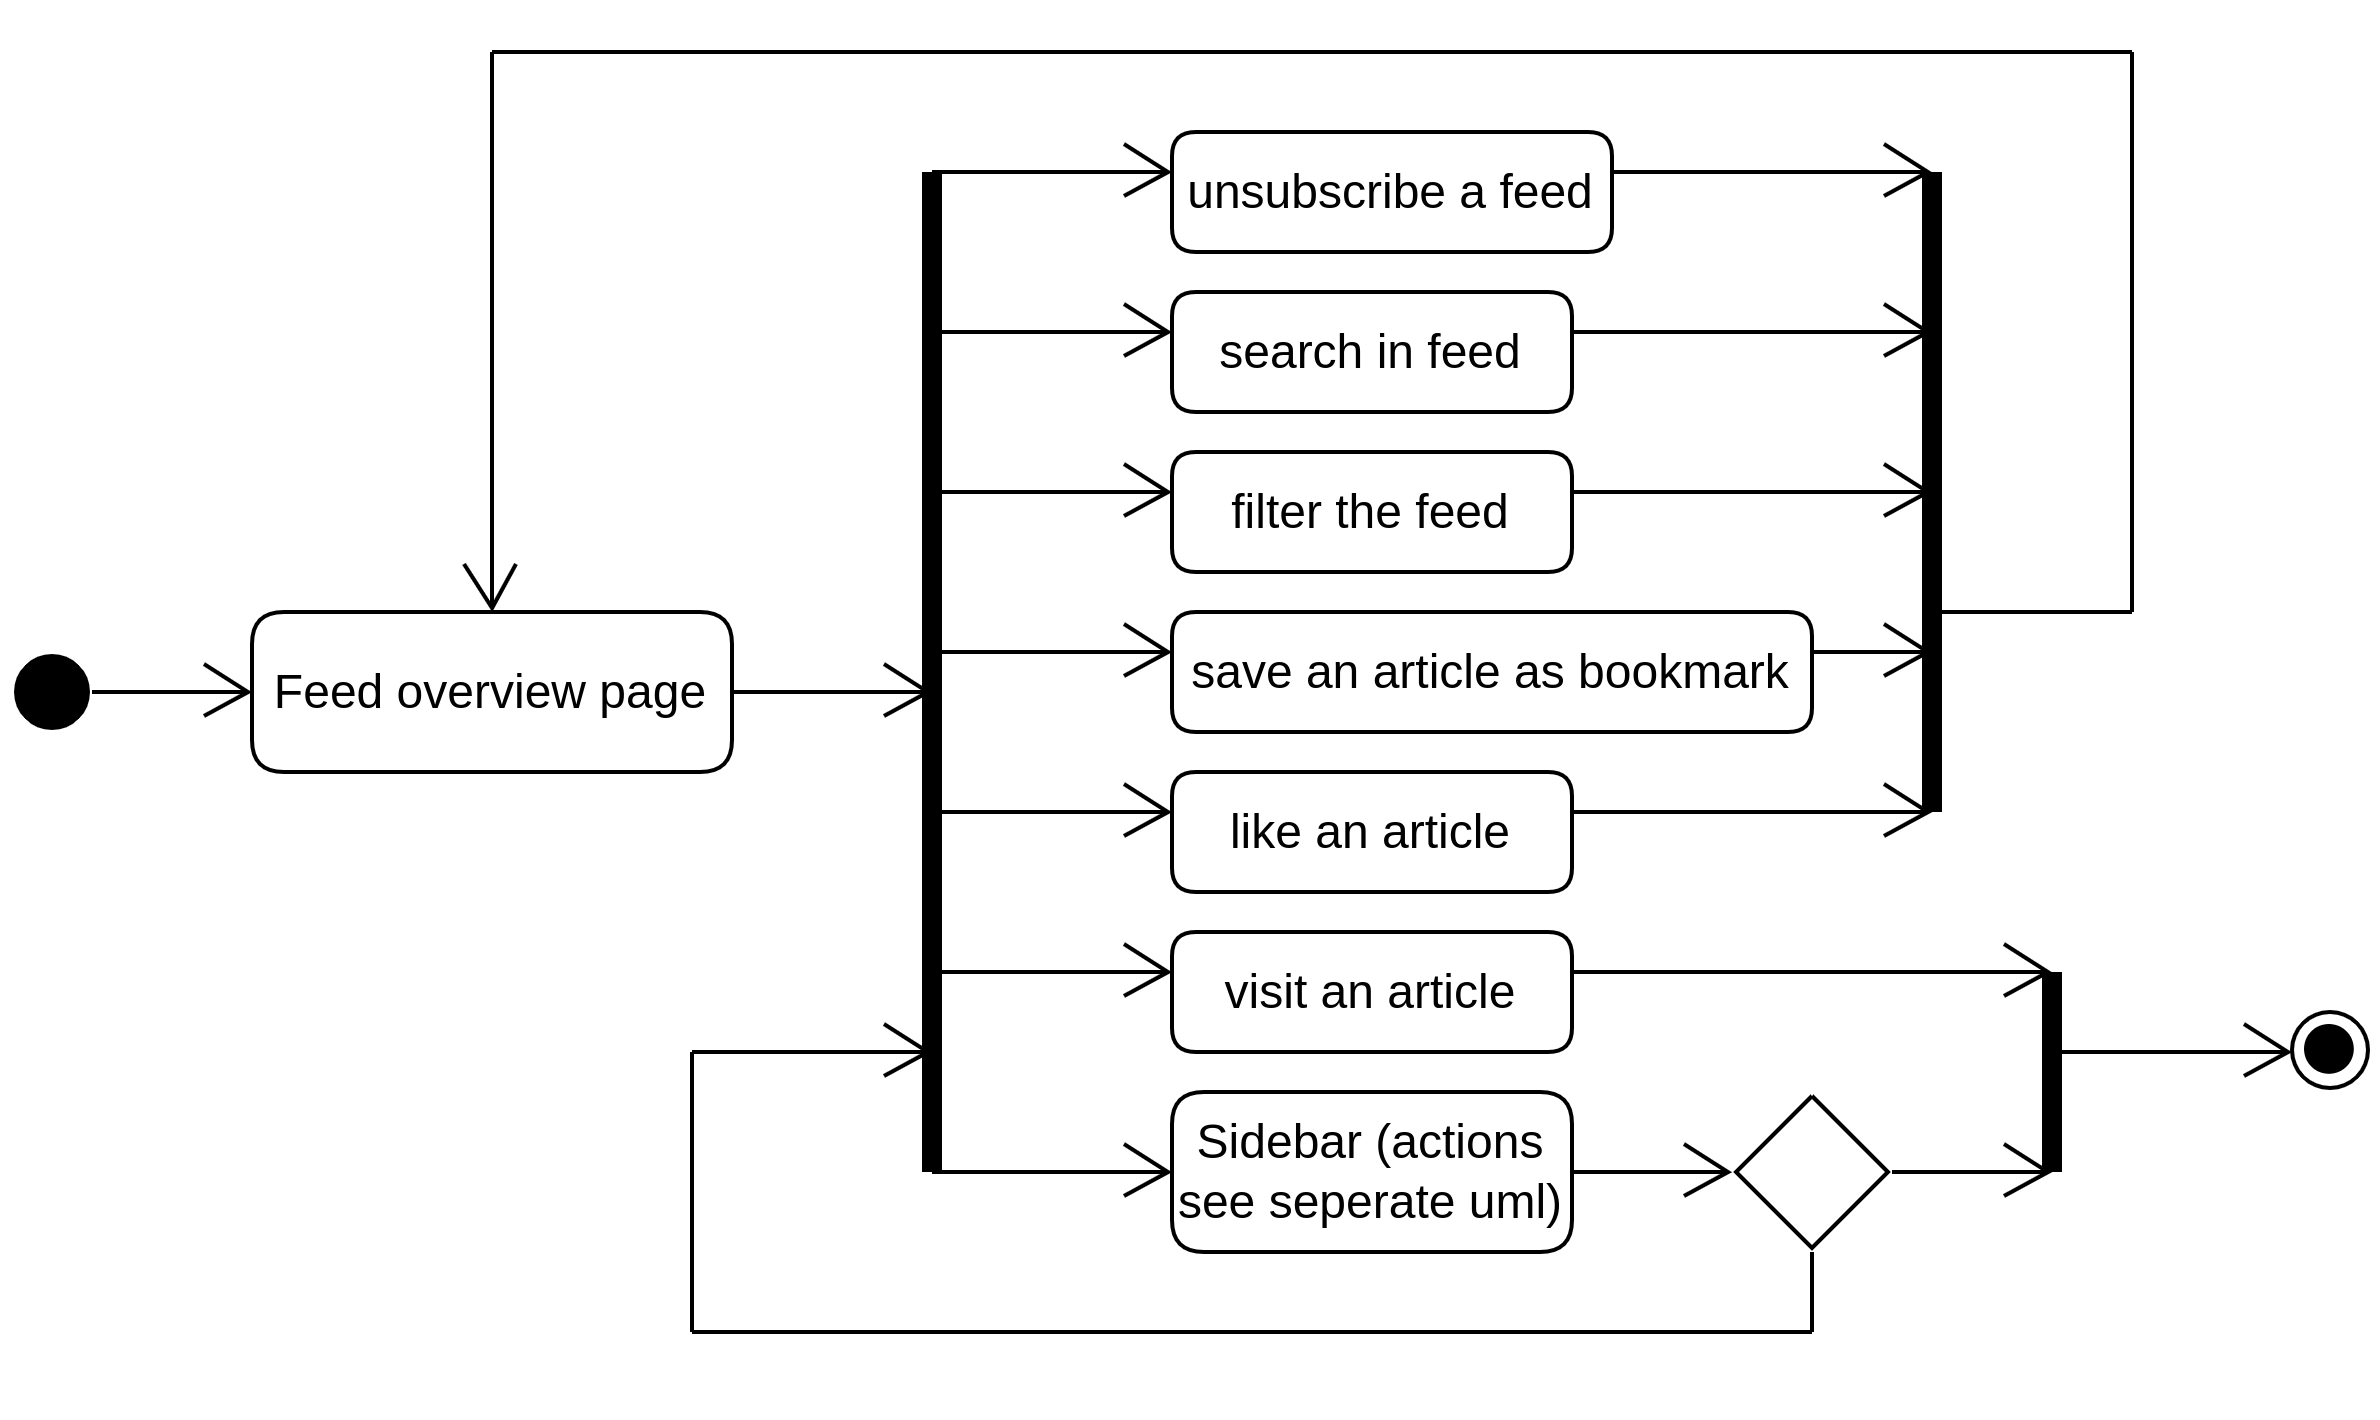
\includegraphics[width=\linewidth]{umlActivityFeed.png}
    \caption{Aktivitätsdiagramm der Feedseite}
    \label{fig:umlActivityFeed.png}
\end{figure}

Auf der Artikelseite kann, wie in Abbildung~\ref{fig:umlActivityView.png} dargestellt der Artikel gelesen werden.
Darüber hinaus kann der Artikel als Lesezeichen gespeichert, geliked und/oder geteilt werden (Link wird in die Zwischenablage kopiert).
Auch die Feedseite des Artikels kann aufgerufen werden. Die Ursprungswebseite des Artikels kann auch geöffnet werden.
Unter den ähnlichen Artikeln kann zu diesem per Klick gewechselt werden.
\begin{figure}
    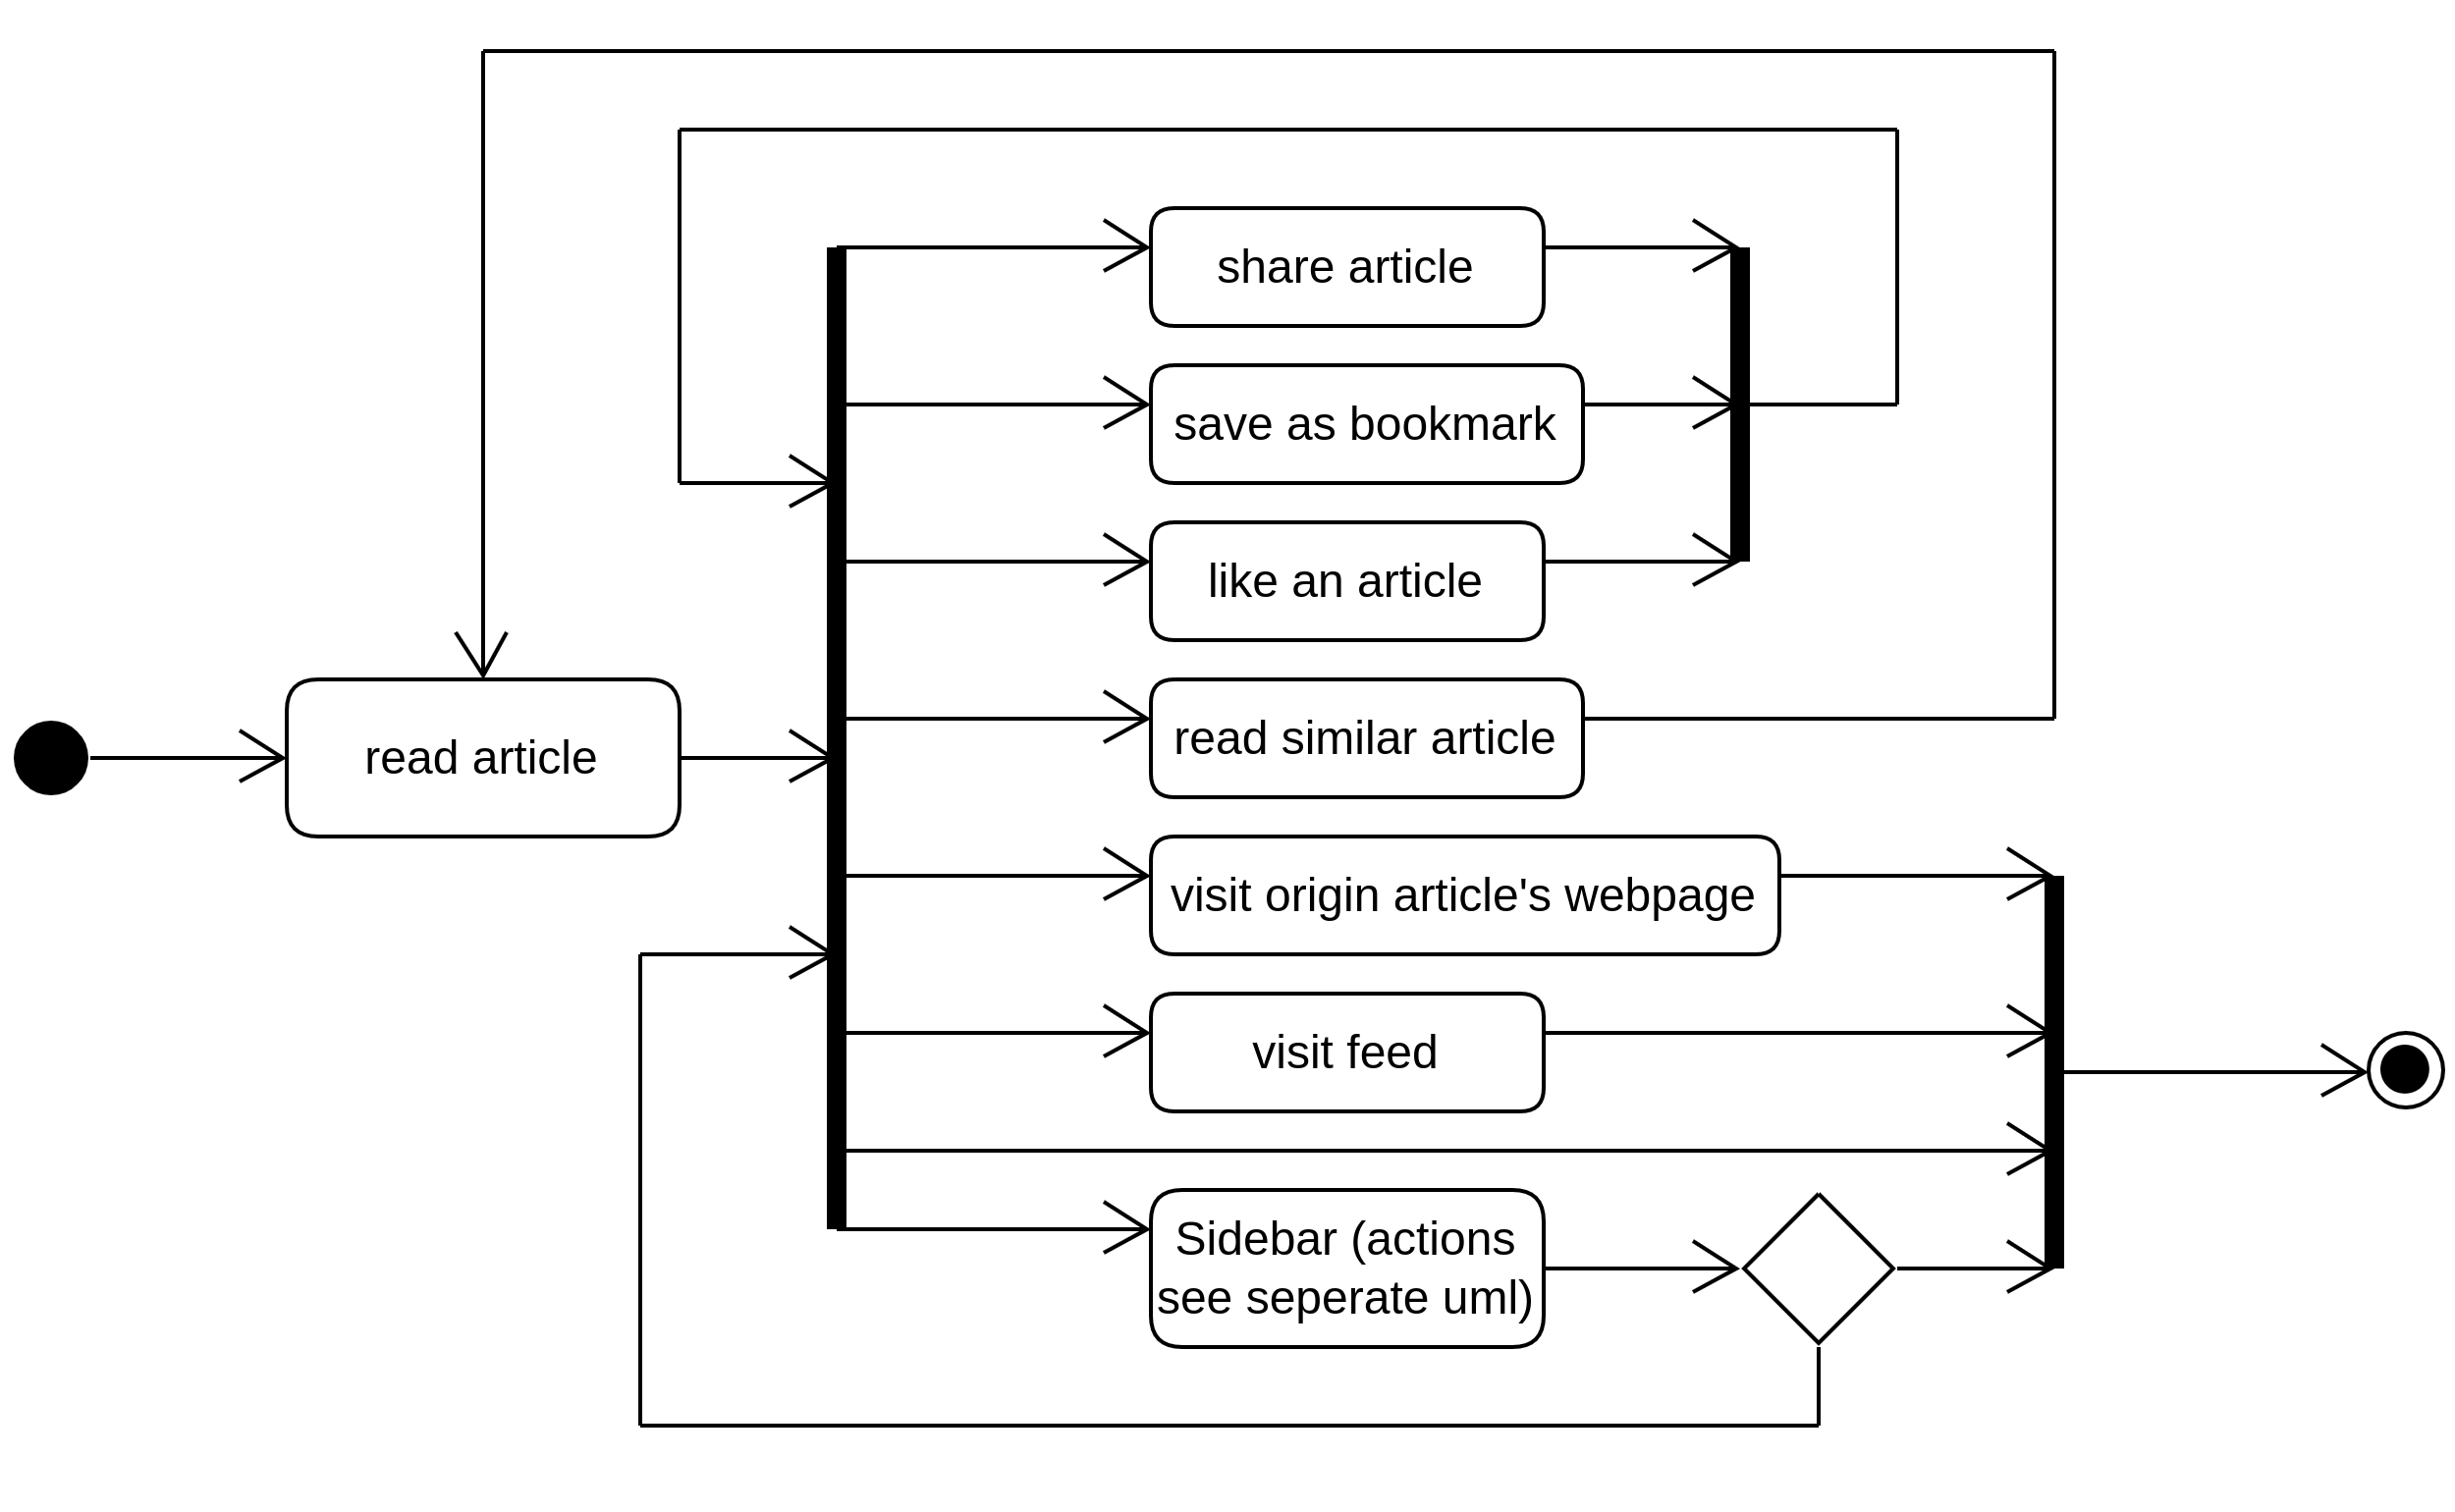
\includegraphics[width=\linewidth]{umlActivityView.png}
    \caption{Aktivitätsdiagramm der Artikelseite}
    \label{fig:umlActivityView.png}
\end{figure}


In Abbildung~\ref{fig:umlActivityBookmarks.png} ist das Aktivitätsdiagramm der Lesezeichenseite dargestellt.
Alle vom Nutzer gespeicherten Lesezeichen werden hier aufgelistet und es kann gefiltert und/ oder darin gesucht werden.
Einzelne Artikel können aus den Lesezeichen gelöscht werden. Auch können einzelne Artikel geliked oder entliked werden.
\begin{figure}
    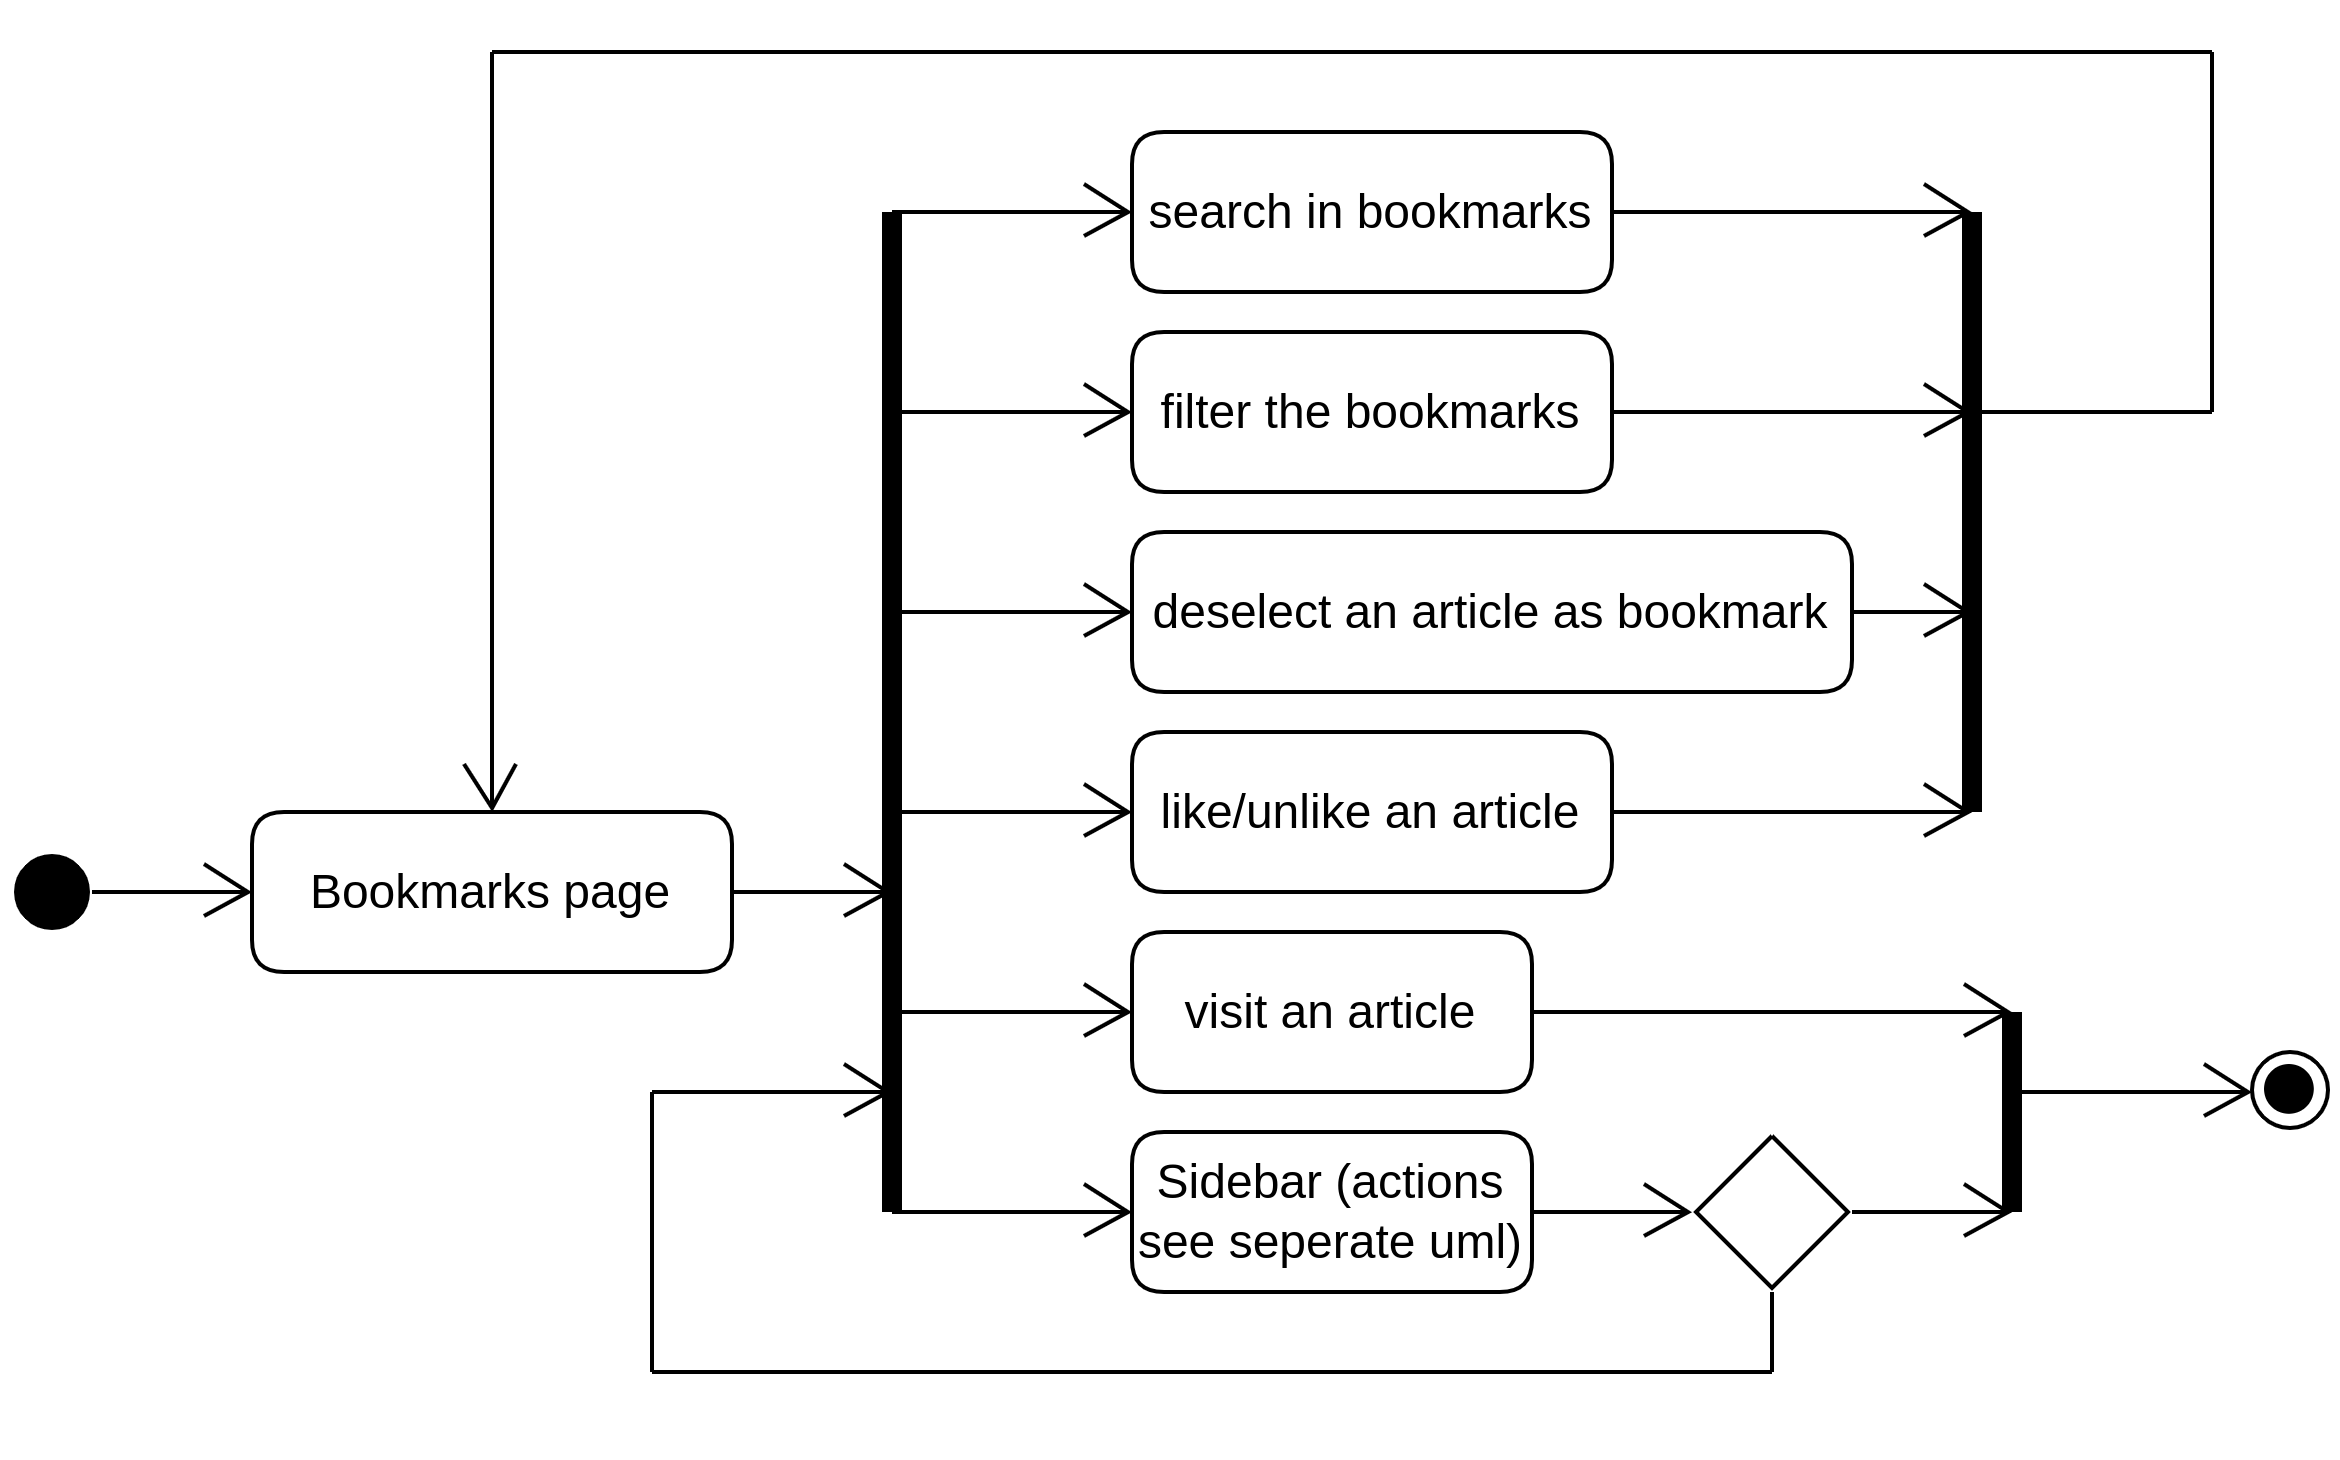
\includegraphics[width=\linewidth]{umlActivityBookmarks.png}
    \caption{Aktivitätsdiagramm der gespeicherten Lesezeichenseite}
    \label{fig:umlActivityBookmarks.png}
\end{figure}

Die Aktivitäten der Abonnementsseite werden in Abbildung~\ref{fig:umlActivitySubscription.png} abgebildet.
Die Abonnements können gefiltert und/oder durchsucht werden. Jeder abonnierte Feed per Klick auf diesen aufgerufen werden.
Ein Feed kann ausgeklappt werden und die 10 aktuellsten Artikel werden angezeigt.
Die gezeigten einzelnen Artikel geliked oder als Lesezeichen gespeichert werden.

Die Artikel können mit einem Klick aufgerufen werden.
\begin{figure}
    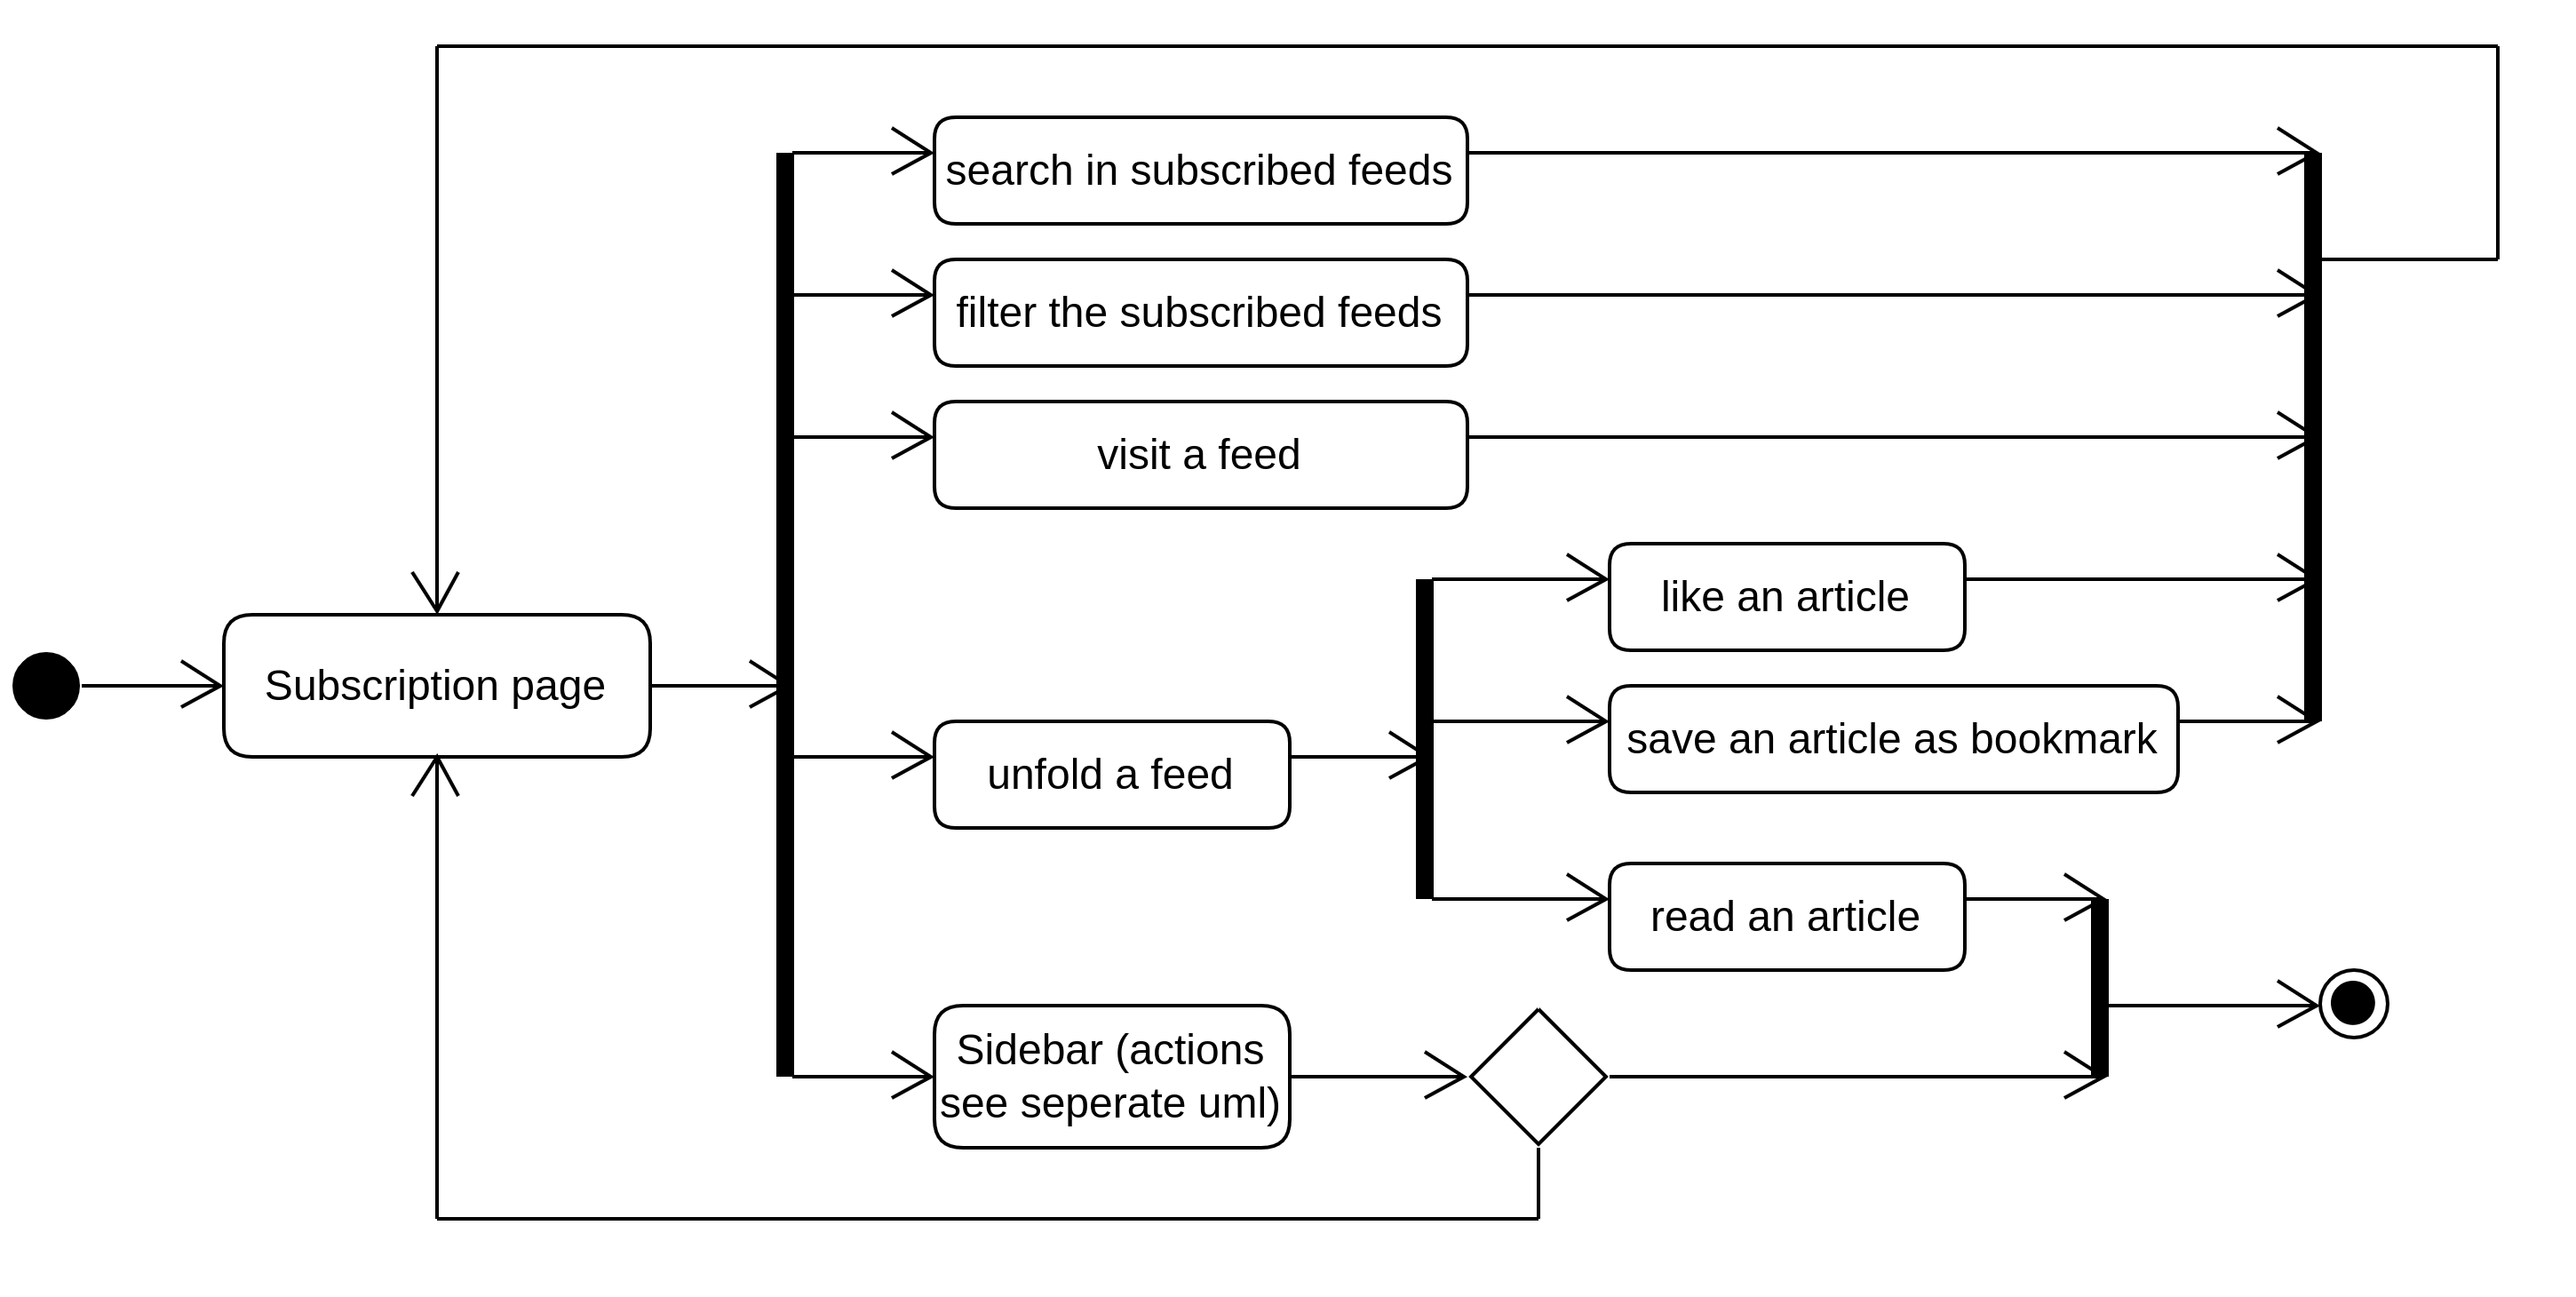
\includegraphics[width=\linewidth]{umlActivitySubscription.png}
    \caption{Aktivitätsdiagramm der Abonnements}
    \label{fig:umlActivitySubscription.png}
\end{figure}

In der Abbildung~\ref{fig:umlActivityAddFeed.png} wird der Ablauf zum Hinzufügen eines neuen Feeds dargestellt.
Ein RSS-Link wird eingetragen und mit klick auf \enquote{load} wird der Link geprüft.
Ist der Link fehlerbehaftet oder entspricht er nicht unserem Schema muss er korrigiert werden.
Funktioniert der Link werden Name und Beschreibung vorausgefüllt.
Der Name und die Beschreibung kann vor dem finalen Hinzufügen noch angepasst werden.
Das Hinzufügen eines Feeds kann jederzeit über die Schaltfläche verlassen werden.
\begin{figure}
    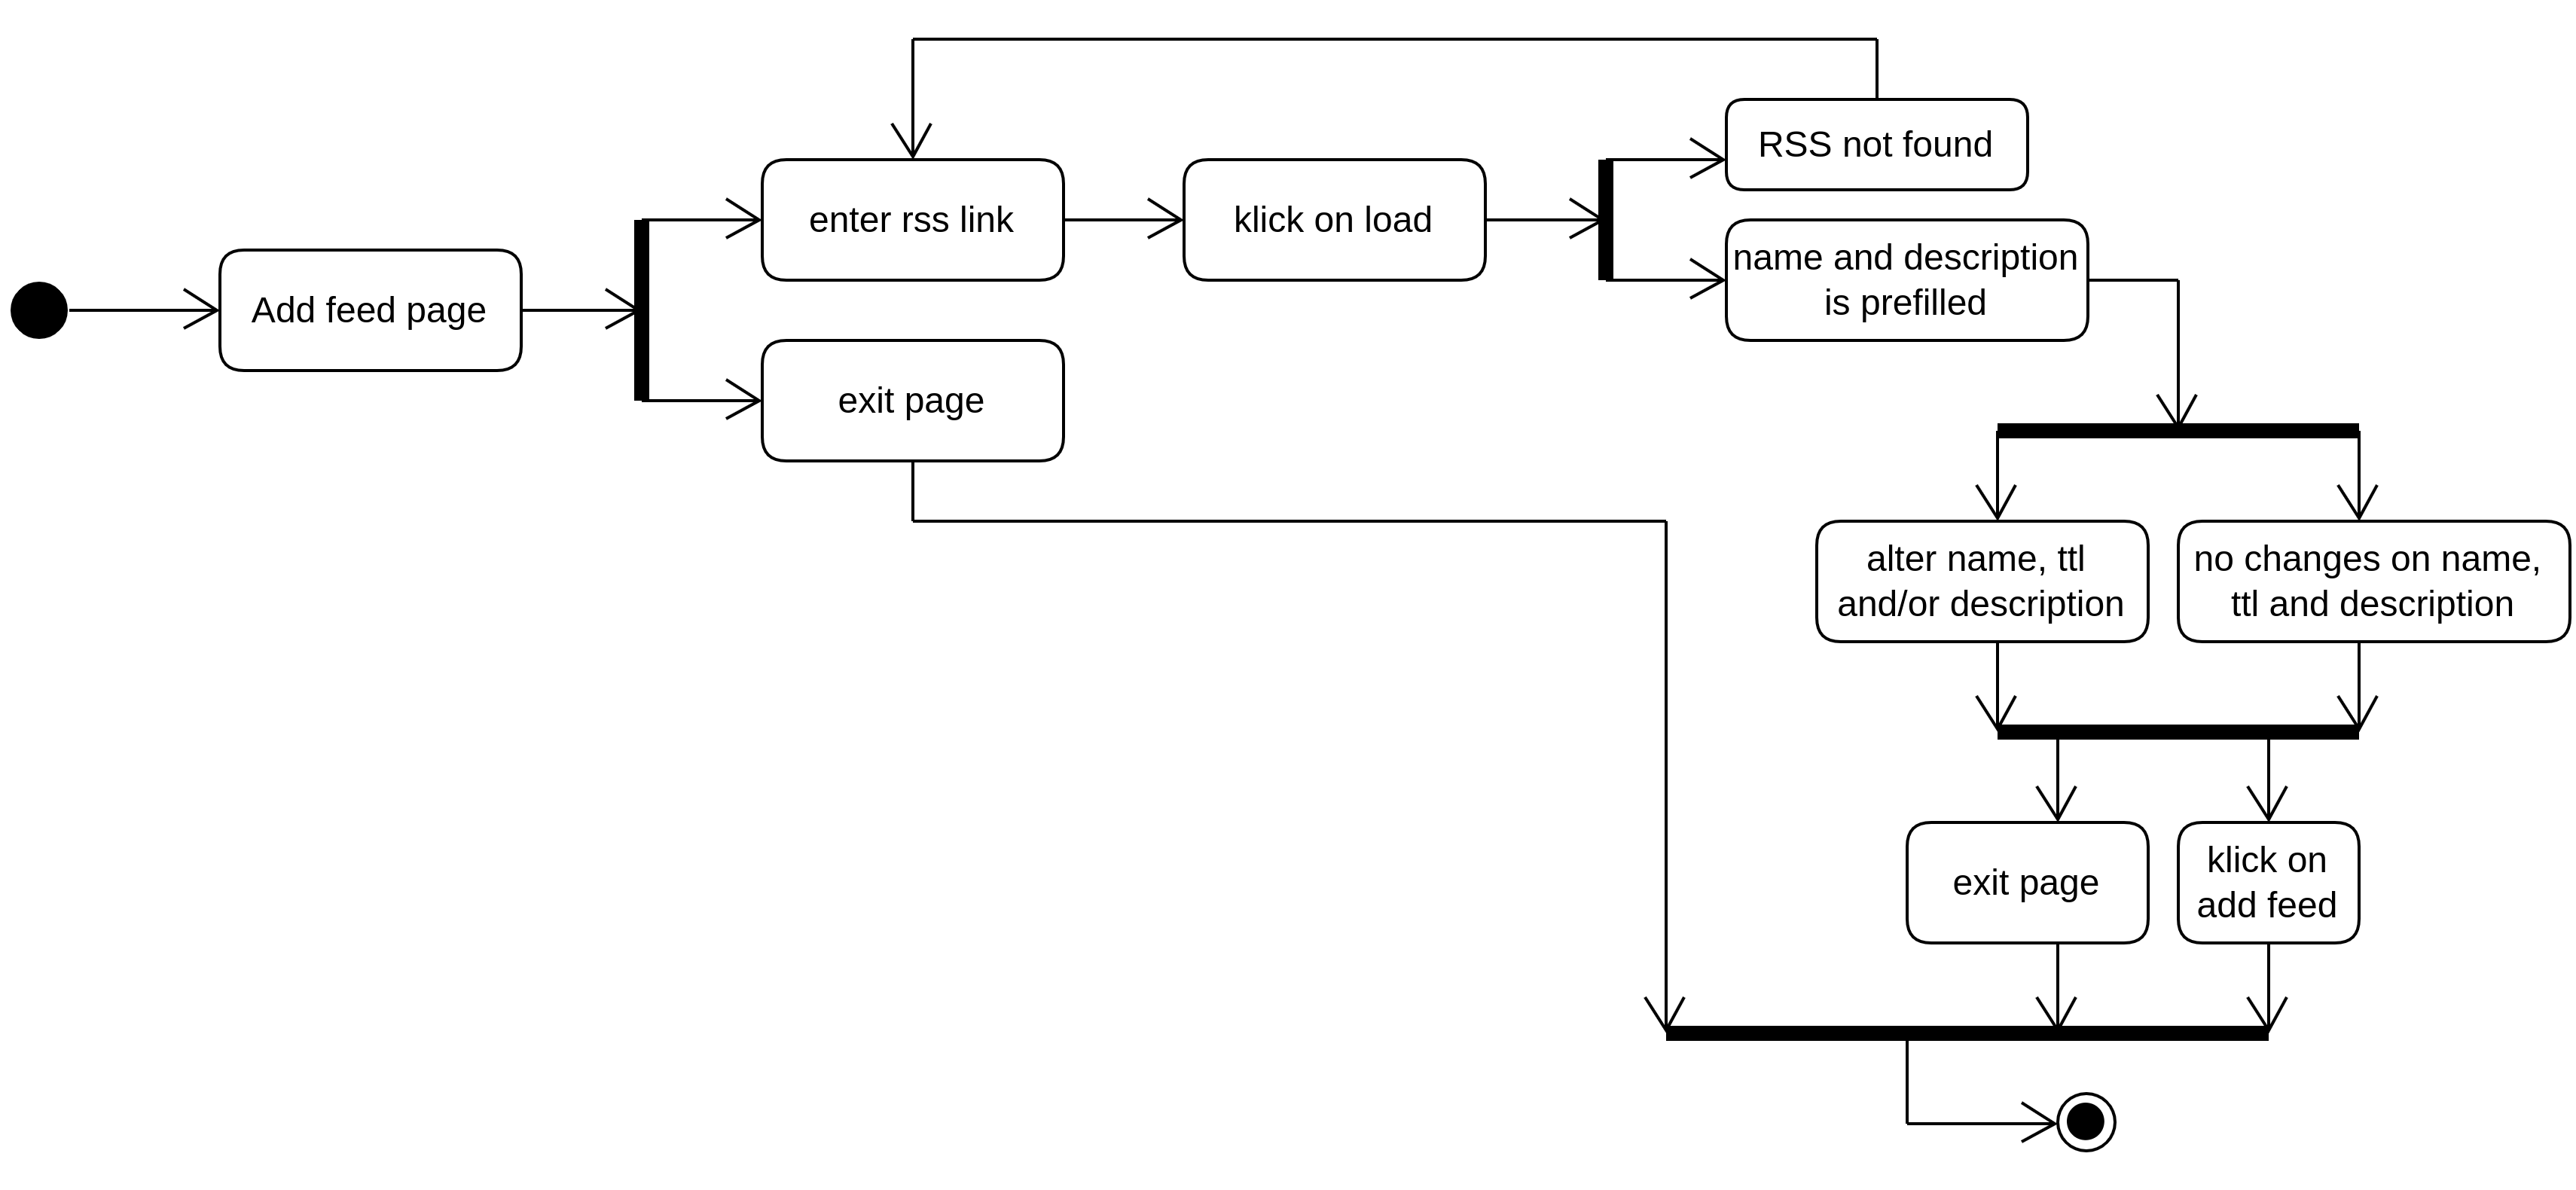
\includegraphics[width=\linewidth]{umlActivityAddFeed.png}
    \caption{Aktivitätsdiagramm zum Hinzufügen eines Feeds}
    \label{fig:umlActivityAddFeed.png}
\end{figure}

Der Nutzer kann die Einstellungen gemäß Abbildung~\ref{fig:umlActivitySettings.png} ändern.
Es können die Accounteinstellungen und das Farbschema angepasst werden.
Ausloggen kann sich der Nutzer in den Einstellungen auch.
\begin{figure}
    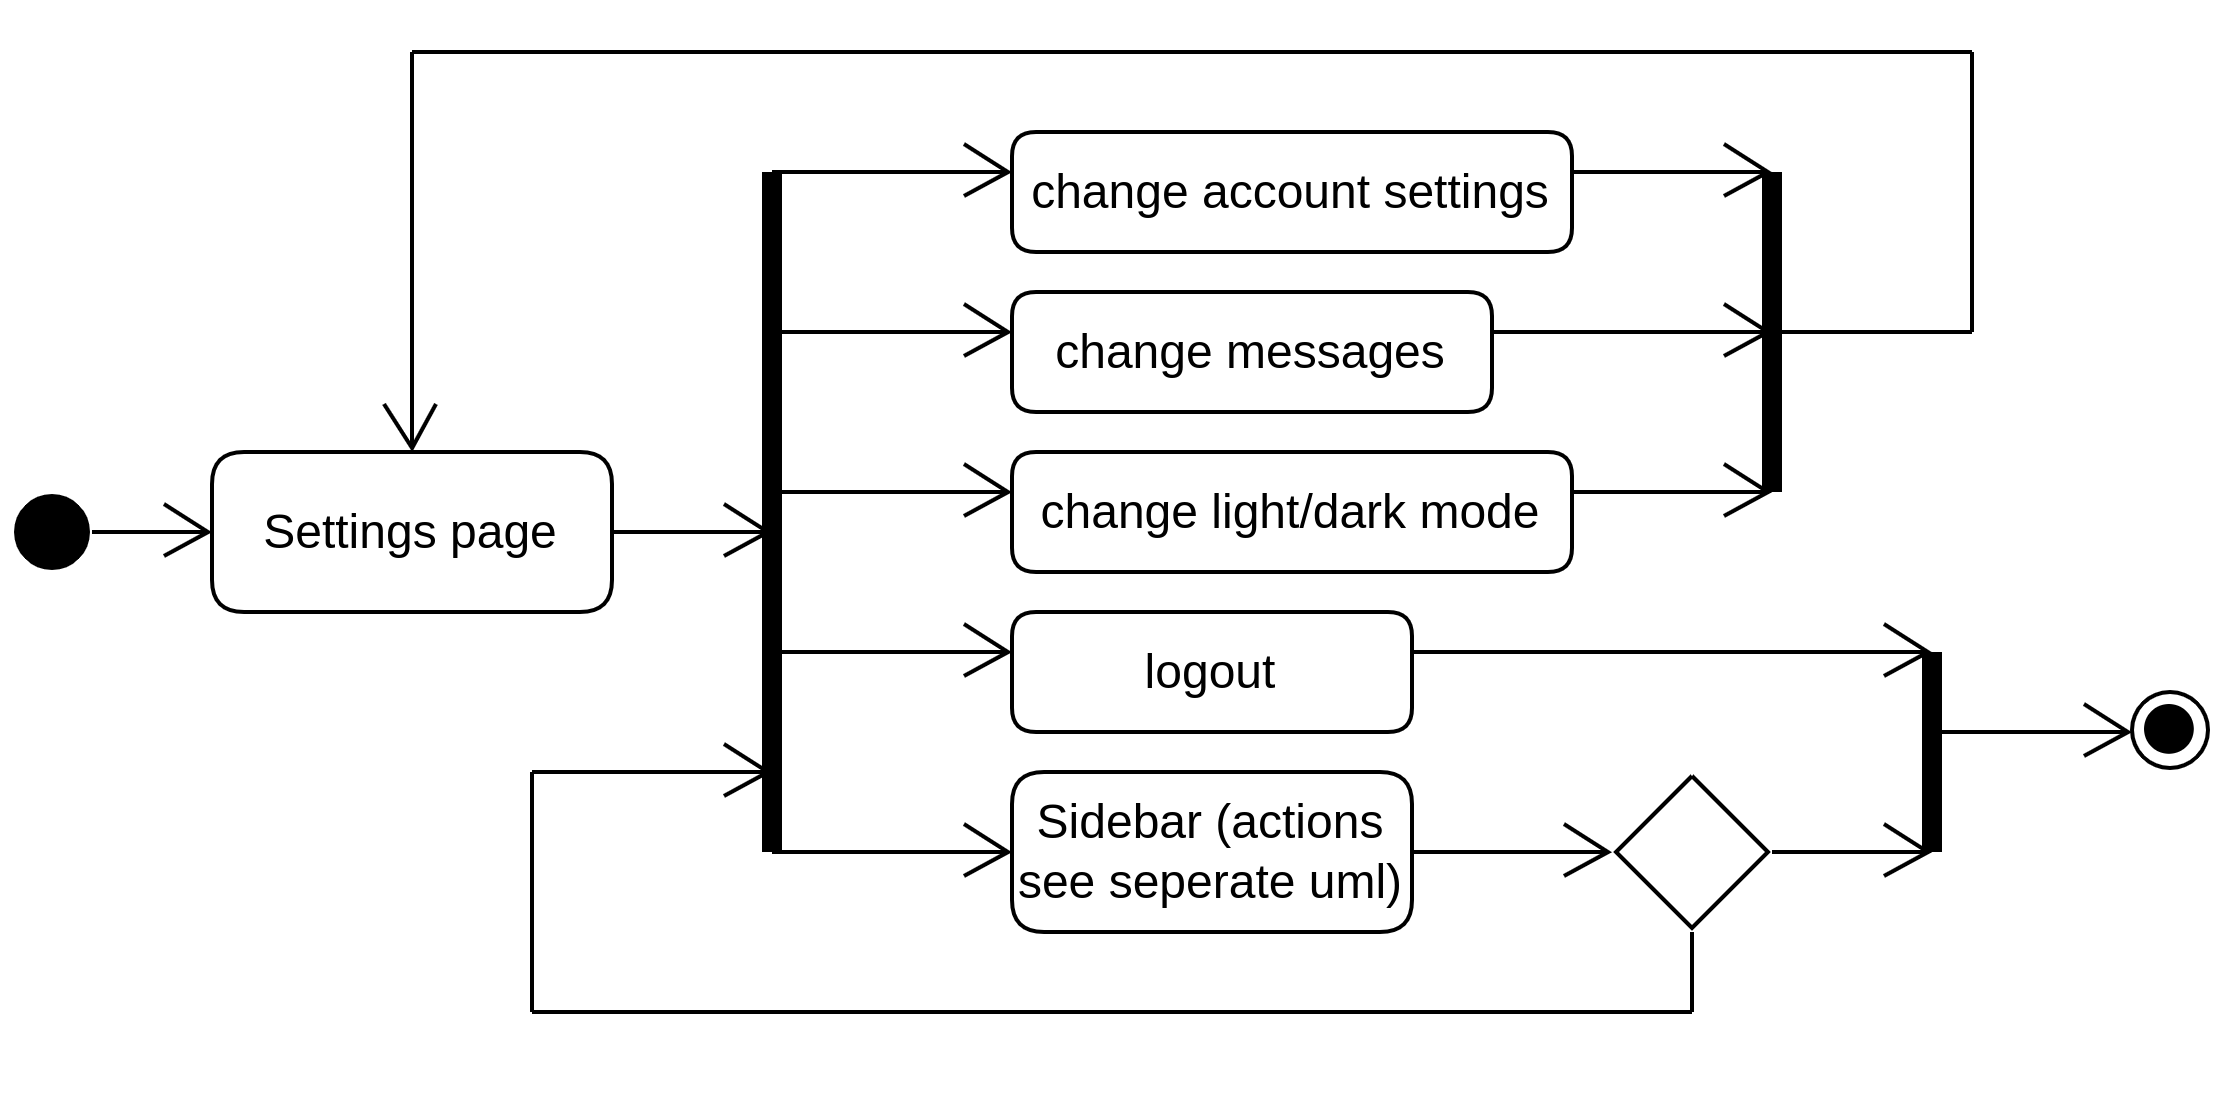
\includegraphics[width=\linewidth]{umlActivitySettings.png}
    \caption{Aktivitätsdiagramm der Einstellungsseite}
    \label{fig:umlActivitySettings.png}
\end{figure}





\section{Technische Änderungen zur anfänglichen Struktur} \label{tech_changes}
Im Laufe unseres Projektes sind einige technischen Hürden entstanden. Diese haben zum Teil dazu geführt das unsere ursprünglichen Requirements nicht mehr erfüllt werden konnten.
Deshalb wurden sie im Nachhinein dementsprechend leicht angepasst.

\begin{table}[h]
    \resizebox{\textwidth}{!}{\begin{tabular}{|p{8cm}|p{8cm}|}
    \hline
    Beschreibung der Änderung & Begründung der Änderung\\ \hline
    In der Plattform soll von RSS Feeds kein Inhalt (bzw. nur eine Beschreibung) angezeigt werden & Ein Großteil der im Internet vohandenen RSS Feeds verlinken nur auf Artikel und enthalten keinen Inhalt. \\ 
    Das Hinzufügen von Feeds aus der Creator Page wurde zu einem Must-Have Requirement & Das anfänglich geplante manuelle Einbinden von Feeds ist als zu zeitaufwändig eingeschätzt worden. \\
    Polling Intervall (TTL) nicht mehr Teil der Creator Page & Ein RSS Feed besitzt bereits ein TTL Feld, durch das dieser Interval bereits angegeben wird. \\
    \hline
\end{tabular}}
\caption{Tabelle – Änderungen zur anfänglichen Struktur}
\end{table}

Wie am Beispiel des RSS Feeds der Tagesschau\footnote{https://www.tagesschau.de/xml/rss2/} zu erkennen ist, liefern viele RSS Feeds einen TTL Wert.
Mit diesem ist zu erkennen, in welchem Intervall der jeweilige Feed neue Informationen bereitstellt. Das mögliches Polling Intervall in der Content-Creator-Page (falls implementiert) wird dadurch redundant.
Zusätzlich ist am obersten Artikel zu sehen, wie im Inhalt nur auf ein Link zur Webseite der Tagesschau verwiesen wird und nicht etwa der Inhalt des Artikels enthalten ist.
So ist es ebenfalls leicht zu erkennen, dass das Anzeigen des Inhalts, wie es in den initialen Requirements enthalten ist, nicht möglich ist.

\begin{lstlisting}[title=Tagesschau RSS Feed,language=xml]
<rss version="2.0">
    <channel>
        <title>tagesschau.de - Die Nachrichten der ARD</title>
        <link>https://www.tagesschau.de</link>
        <description>tagesschau.de</description>
        <language>de</language>
        <copyright>ARD-aktuell / tagesschau.de</copyright>
        <lastBuildDate>Tue, 03 May 2022 16:54:20 +0200</lastBuildDate>
        <docs>http://blogs.law.harvard.edu/tech/rss</docs>
        <ttl>10</ttl>
        <item>
            <title>Marktbericht: Anleger wagen sich noch etwas vor</title>
            <link>
            https://www.tagesschau.de/wirtschaft/finanzen/marktberichte/boerse-marktbericht-dax-dow-jones-101.html
            </link>
            <pubDate>Tue, 03 May 2022 18:10:20 +0200</pubDate>
            <description>
            Nach meist richtungslosem Handel kam am Ende des Tages doch noch etwas Interesse auf. Die Anleger warten derweil mit Spannung auf die Ergebnisse der Zinssitzung der US-Notenbank.
            </description>
            <guid>
            https://www.tagesschau.de/wirtschaft/finanzen/marktberichte/boerse-marktbericht-dax-dow-jones-101.html
            </guid>
            <content:encoded>
            <p> <a href="https://www.tagesschau.de/wirtschaft/finanzen/marktberichte/boerse-marktbericht-dax-dow-jones-101.html"><img src="https://www.tagesschau.de/multimedia/bilder/boerse-frankfurt-141~_v-mittel16x9.jpg"/></a> <br/> <br/> Nach meist richtungslosem Handel kam am Ende des Tages doch noch etwas Interesse auf. Die Anleger warten derweil mit Spannung auf die Ergebnisse der Zinssitzung der US-Notenbank. <a href="https://www.tagesschau.de/wirtschaft/finanzen/marktberichte/boerse-marktbericht-dax-dow-jones-101.html">mehr</a> </p> <ul> </ul> </p> <p><a href="https://www.tagesschau.de/wirtschaft/finanzen/marktberichte/boerse-marktbericht-dax-dow-jones-101.html">Meldung bei www.tagesschau.de lesen</a></p>
            </content:encoded>
        </item>
    </channel>
</rss>
\end{lstlisting}
